	\chapter{Hierarchical Clustering and PCA}
	\resetquestioncounter{}
	\begin{qanda}
		\begin{question}
PCA explained how to reduce dimensions on the data set, However, when solved, there is no info on which dimensions (columns) are the most important and which we can remove. How can I know that information?
		\end{question}
		\begin{answer}
Using PCA, the columns are completely changed. PCA finds a new relationship between the columns. So, we use it to get a higher score. If the focus is to find feature importance, then PCA fails as it completely transforms the columns and new columns will not mean the same as the older ones, so we cannot name them. Feature importance after PCA will make no sense at all.

After transforming columns using PCA we try to take the minimum number of columns through which we can achieve the maximum score.
		\end{answer}
	\end{qanda}


	\begin{qanda}
		\begin{question}
How do we choose the correct distance to use in clustering algorithms?
		\end{question}
		\begin{answer}
There is no single distance that will give the best results with all data and all problem statements. The type of distance you use depends on the data and the problem statement. Generally normalized Euclidean distance is used. However, when data size is very large and high dimensional, Manhattan distance is found to perform better computationally. The type of distance to use is decided by the problem at hand.
		\end{answer}
	\end{qanda}


	\begin{qanda}
		\begin{question}
What then do we do with the clusters after interpretations?
		\end{question}
		\begin{answer}
What you do with clusters after interpretation depends upon the problem you are trying to solve. Clustering will give you groups that are similar in some aspects. This can be used for recommendations, understanding customers, market campaigning, etc. Again what you do after interpretation of clustering depends upon what problem you are trying to solve.
		\end{answer}
	\end{qanda}

	\begin{qanda}
		\begin{question}
How do we know whether K-means or hierarchical clustering is appropriate to use in a given business problem?
		\end{question}
		\begin{answer}
The k-means algorithm is used when it is already known in advance how many clusters have to be formed, also k-means is suitable if your data is well separated into spherical-like clusters. On the other hand, hierarchical clustering is density-based clustering in which nearby points are joined to form clusters. It gives you a dendrogram from which you can figure out how many clusters should be formed. Hierarchical clustering is computationally expensive so it will not perform well when the data size is very very big.
		\end{answer}
	\end{qanda}

	\begin{qanda}
		\begin{question}
I get the following error when I try to use SilhouetteVisualizer with AgglomerativeClustering.
AttributeError: `AgglomerativeClustering' object has no attribute `predict'
Why does this throw the error and how to debug this?
		\end{question}
		\begin{answer}
The SilhouetteVisualizer function from yellowbrick library is designed for visualizing the cluster of K-means only as you can read from its documentation. If you want to find the silhouette score for clusters obtained using hierarchical clustering, then you have to use sklearn function of silhouette score which is given here.

A sample code is given below

score = silhouette\_score(X, HCmodel.labels\_, metric=`euclidean')
where X is a scaled dataset, and HCmodel is the agglomerative model fit on the data set.
		\end{answer}
	\end{qanda}

	\begin{qanda}
		\begin{question}
Are correlated features a problem when it comes to clustering? If so can you point me to why this might be a problem?
		\end{question}
		\begin{answer}
First of all, you have to decide which variables you should be used for clustering, Once you have done that, it is better to choose only those variables among them, such that no two variables have a correlation of more than 0.7 (magnitude).

Correlation does not have a negative impact on clustering but removing correlated variables helps to reduce the dimension and can be computationally efficient when you have a very large number of observations.
		\end{answer}
	\end{qanda}

	\begin{qanda}
		\begin{question}
How do we select the optimal number of clusters from the Dendrogram?
		\end{question}
		\begin{answer}
Choosing the optimal number of clusters is a fairly subjective matter, and the best method to identify the optimum number of clusters is to use a combination of metrics and domain expertise. The dendrogram is one of the most common ways for estimating the appropriate number of clusters for hierarchical clustering if we don't have domain expertise.

The optimal number of clusters from a dendrogram can be obtained by deciding where to cut the cluster tree. Generally, the cluster tree is cut where the dendrogram height is maximum as it corresponds to distinct and homogeneous clusters.

Please refer to the \figurename~\ref{fig:hierarchicalclustering} for an example, the distance between the red horizontal lines denotes the maximum distance that has been traversed without intersecting any cluster. So, the ideal number of clusters, from the above dendrogram can be 4 clusters. However, one should also do cluster profiling and check if the cluster profiles are meaningful and have variability, for which domain knowledge is needed.

We can get a different number of clusters from the dendrogram at different heights. But the standard approach to picking the appropriate number of clusters from the dendrogram is to check the maximum height of the vertical line formed.
		\end{answer}
	\end{qanda}

	\begin{figure}[h]
		\centering
		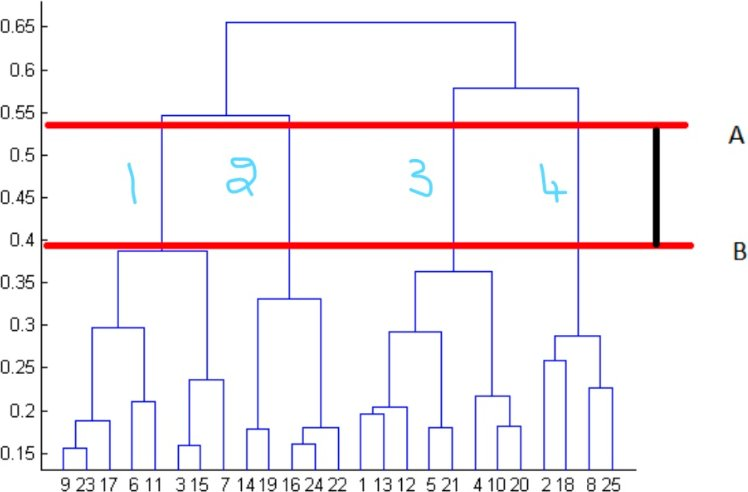
\includegraphics[height=2.0in]{hierarchicalclustering}
		\caption{Normal distribution.}
		\label{fig:hierarchicalclustering}
	\end{figure}